\documentclass[11pt,a4paper]{article}

\usepackage[a4paper,margin=1in]{geometry}
\usepackage{amsmath,amssymb}
\usepackage{graphicx}
\usepackage[hidelinks]{hyperref}
\usepackage{float}
\usepackage{tikz}
\usetikzlibrary{calc,decorations.pathreplacing}

% Partial-overlap figure, computed from the parameters.
% #1 = p, #2 = z, #3 = drawing scale, #4 = placement of the O_2 label,
% #5 = side of the line O_2B on which the p r_* label sits (above/below),
% #6 = position of the r_* label along O_1B (0 = at O_1, 1 = at B).
% Stellar radius is 1.
\newcommand{\overlapfigure}[6]{%
\begin{tikzpicture}[scale=#3, font=\small]
  \pgfmathsetmacro{\ovp}{#1}
  \pgfmathsetmacro{\ovz}{#2}
  \pgfmathsetmacro{\ova}{acos((\ovz*\ovz-\ovp*\ovp+1)/(2*\ovz))}
  \pgfmathsetmacro{\ovb}{acos((\ovz*\ovz+\ovp*\ovp-1)/(2*\ovp*\ovz))}
  \coordinate (O1) at (0,0);
  \coordinate (O2) at (\ovz,0);
  \coordinate (A)  at ({\ovz-\ovp},0);
  \coordinate (C)  at (1,0);
  \coordinate (B)  at ({cos(\ova)},{sin(\ova)});
  \coordinate (D)  at ({cos(\ova)},0);
  % regions S1 (planet segment on AB), S2 (triangle ABC), S3 (star segment on BC)
  \fill[orange!45]  (A) arc[start angle=180, end angle={180-\ovb}, radius=\ovp] -- cycle;
  \fill[green!35]   (A) -- (B) -- (C) -- cycle;
  \fill[magenta!40] (C) arc[start angle=0, end angle=\ova, radius=1] -- cycle;
  % the two bodies and the axis
  \draw[thick] (O1) circle[radius=1];
  \draw[thick] (O2) circle[radius=\ovp];
  \draw[gray] (-1.1,0) -- ({\ovz+\ovp+0.1},0);
  % construction lines
  \draw[teal!70!black] (O1) -- node[pos=#6, sloped, above]{$r_*$} (B);
  \draw[teal!70!black] (O2) -- node[pos=0.3, sloped, #5]{$p r_*$} (B);
  \draw[violet] (A) -- (B) -- (C);
  \draw[red] (B) -- (D);
  % angles
  \draw[red] (0.15,0) arc[start angle=0, end angle=\ova, radius=0.15];
  \node[red] at ({0.27*cos(\ova/2)},{0.27*sin(\ova/2)}) {$\alpha$};
  \draw[red] ($(O2)+(-0.15,0)$) arc[start angle=180, end angle={180-\ovb}, radius=0.15];
  \node[red] at ($(O2)+({0.27*cos(180-\ovb/2)},{0.27*sin(180-\ovb/2)})$) {$\beta$};
  % points
  \foreach \pt in {O1,O2,A,B,C,D} \fill (\pt) circle[radius=0.02];
  \node[below right] at (O1) {$O_1$};
  \node[#4] at (O2) {$O_2$};
  \node[below left]  at (A)  {$A$};
  \node[below]       at (D)  {$D$};
  \node[below right] at (C)  {$C$};
  \node[above]       at (B)  {$B$};
  % separation
  \draw[decorate, decoration={brace, mirror, amplitude=4pt}]
    (0,-0.3) -- (\ovz,-0.3) node[midway, below=4pt] {$z r_*$};
  % region and body labels
  \node at ($(O2)+({(\ovp+0.1)*cos(180-\ovb/2)},{(\ovp+0.1)*sin(180-\ovb/2)})$) {$S_1$};
  \node at ({(\ovz-\ovp+cos(\ova)+1)/3},{sin(\ova)/3}) {$S_2$};
  \node at ({1.1*cos(\ova/2)},{1.1*sin(\ova/2)}) {$S_3$};
  \node at ({1.15*cos(220)},{1.15*sin(220)}) {star};
  \node at ($(O2)+({(\ovp+0.15)*cos(300)},{(\ovp+0.15)*sin(300)})$) {planet};
\end{tikzpicture}}

\title{\texttt{transit-lab}: Technical Report}
\author{Roman}
\date{}

\begin{document}

\maketitle
\tableofcontents
\newpage

\section{Introduction}
\label{sec:introduction}

\section{Background}
\label{sec:background}

\section{Methods}
\label{sec:methods}

\section{Results}
\label{sec:results}

\section{Failure analysis}
\label{sec:failure-analysis}

\section{Limitations}
\label{sec:limitations}

\section{Conclusion}
\label{sec:conclusion}

\appendix

\section{Derivations}
\label{sec:app-derivations}

% ---------------------------------------------------------------------------
\subsection{Conventions}
\label{sec:app-conventions}

\begin{figure}[H]
  \centering
  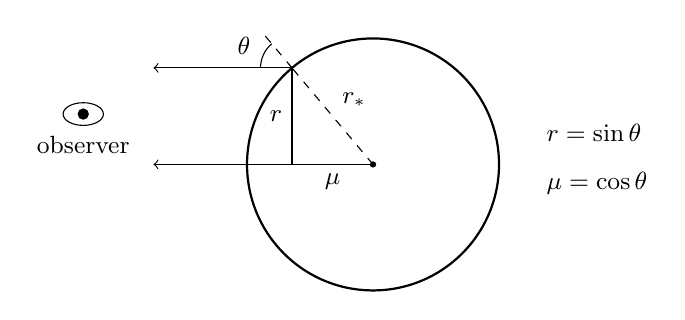
\begin{tikzpicture}[scale=1.6, font=\small]
    \pgfmathsetmacro{\th}{50}
    \coordinate (O) at (0,0);
    \coordinate (P) at ({-cos(\th)},{sin(\th)});
    \coordinate (F) at ({-cos(\th)},0);
    \draw[thick] (O) circle[radius=1];
    \fill (O) circle[radius=0.025];
    % radius and outward normal at P
    \draw[dashed] (O) -- node[above right]{$r_*$} (P);
    \draw[dashed] (P) -- ($(O)!1.35!(P)$);
    % rays towards the observer
    \draw[->] (P) -- ++(-1.1,0);
    \draw[->] (F) -- ++(-1.1,0);
    % projected radius r and depth coordinate mu
    \draw (P) -- node[left]{$r$} (F);
    \draw (F) -- node[below]{$\mu$} (O);
    % theta between the normal and the line of sight
    \draw ($(P)+(180-\th:0.25)$) arc[start angle={180-\th}, end angle=180, radius=0.25];
    \node at ($(P)+({180-\th/2}:0.42)$) {$\theta$};
    % observer
    \draw (-2.3,0.4) ellipse[x radius=0.16, y radius=0.09];
    \fill (-2.3,0.4) circle[radius=0.045];
    \node[below] at (-2.3,0.3) {observer};
    \node[right] at (1.3,0.25)  {$r = \sin\theta$};
    \node[right] at (1.3,-0.15) {$\mu = \cos\theta$};
  \end{tikzpicture}
  \caption{Side view of the star, sliced through its centre, with the observer
  to the left. A point on the stellar surface is at angle $\theta$ between its
  surface normal and the line of sight; its projected distance from the centre
  is $r$, and $\mu$ is the corresponding depth coordinate.}
  \label{fig:conventions}
\end{figure}

With the stellar radius normalised to $1$,
\begin{equation}
  r = \sin\theta, \qquad \mu = \cos\theta .
\end{equation}
\begin{itemize}
  \item $\mu$ is for the physics of limb darkening: it determines at what
        depth the photons we receive are coming out.
  \item $r$ is needed for the geometry: it is how far from the stellar centre
        the light is coming from.
\end{itemize}

Let $d$ be the distance between the centres of the star and the planet, $r_*$
the stellar radius and $r_p$ the planetary radius. Define
\begin{equation}
  z = \frac{d}{r_*}, \qquad p = \frac{r_p}{r_*}.
\end{equation}

Flux is energy per unit time per unit detector area. The most flux the observer
receives is out of transit; when a transit occurs, the flux drops. For light
curves we record the normalised flux $F$, the received flux divided by the
out-of-transit flux.

% ---------------------------------------------------------------------------
\subsection{Occulted area of two overlapping discs}
\label{sec:app-geometry}

\paragraph{Uniform source.}
This assumes the whole area of the star emits light equally, so
\begin{equation}
  F = 1 - \frac{\text{area of overlap}}{\pi r_*^2}.
\end{equation}
Everything in the model is normalised, so only the relative size of the two
bodies ($p$) and their relative separation ($z$) matter. We can therefore write
\begin{equation}
  F^{e}(p,z) = 1 - \lambda^{e}(p,z),
\end{equation}
where $e$ stands for eclipse and $\lambda^{e}$ is the overlap function.

\paragraph{Case 1: no overlap.}
There is no overlap if
\begin{equation}
  d > r_p + r_* \iff z r_* > p r_* + r_* \iff 1 + p < z .
\end{equation}
So $\lambda^{e}(p,z) = 0$ and $F^{e}(p,z) = 1$ here.

\paragraph{Case 2: planet fully inside the star.}
This happens when
\begin{equation}
  d \le r_* - r_p \iff z r_* \le r_* - p r_* \iff z \le 1 - p,
  \qquad \text{with } p < 1 .
\end{equation}
Then
\begin{equation}
  \frac{\text{area of overlap}}{\pi r_*^2} = \frac{\pi r_p^2}{\pi r_*^2} = p^2,
\end{equation}
so $\lambda^{e}(p,z) = p^2$ and $F^{e}(p,z) = 1 - p^2$.

\paragraph{Case 3: star fully inside the planet.}
This happens when
\begin{equation}
  d \le r_p - r_* \iff z \le p - 1, \qquad \text{with } p \ge 1 .
\end{equation}
Then
\begin{equation}
  \frac{\text{area of overlap}}{\pi r_*^2} = \frac{\pi r_*^2}{\pi r_*^2} = 1,
\end{equation}
so $\lambda^{e}(p,z) = 1$ and $F^{e}(p,z) = 0$.

\paragraph{Case 4: partial overlap.}
This is the most thorough case, and whether $p > 1$ or $p \le 1$ does not
matter. It is the only remaining case, so
\begin{equation}
  \underbrace{z > 1 - p > 0}_{p < 1}
  \quad\text{and}\quad
  \underbrace{z > p - 1 \ge 0}_{p \ge 1}
  \quad\text{and}\quad
  z \le 1 + p .
\end{equation}
The first two conditions combine into $z > |1 - p|$, hence
\begin{equation}
  |1 - p| < z \le 1 + p .
\end{equation}

There are three configurations, all sharing the decomposition
$S_1 + S_2 + S_3$ (Figures~\ref{fig:overlap-1}--\ref{fig:overlap-3}).

\begin{figure}[H]
  \centering
  \overlapfigure{0.8}{1.3}{3}{below right}{above}{0.35}
  \caption{Case 4, configuration 1: $\alpha$ and $\beta$ both acute
  (drawn with $p = 0.8$, $z = 1.3$). The star (centre $O_1$, radius $r_*$) and
  the planet (centre $O_2$, radius $p r_*$) have centres a distance $z r_*$
  apart. $B$ is an intersection point of the two circles; $A$ is where the
  planet's boundary meets the axis $O_1O_2$ inside the star; $C$ is where the
  star's boundary meets the axis inside the planet; $D$ is the foot of the
  perpendicular from $B$. The upper half of the overlap is split into the
  planet segment $S_1$ on chord $AB$, the triangle $S_2 = ABC$, and the star
  segment $S_3$ on chord $BC$.}
  \label{fig:overlap-1}
\end{figure}

\begin{figure}[H]
  \centering
  \overlapfigure{0.75}{0.5}{3.2}{below left}{below}{0.35}
  \caption{Case 4, configuration 2: $\beta$ obtuse, with the planet's centre
  $O_2$ inside the star (drawn with $p = 0.75$, $z = 0.5$).}
  \label{fig:overlap-2}
\end{figure}

\begin{figure}[H]
  \centering
  \overlapfigure{1.8}{1.2}{2.2}{below right}{below}{0.7}
  \caption{Case 4, configuration 3: $p > 1$ and $\alpha$ obtuse
  (drawn with $p = 1.8$, $z = 1.2$).}
  \label{fig:overlap-3}
\end{figure}

Let $\alpha = \angle BO_1O_2$ and $\beta = \angle BO_2O_1$. By the cosine rule
in triangle $O_1BO_2$:
\begin{align}
  (p r_*)^2 &= r_*^2 + z^2 r_*^2 - 2 z r_*^2 \cos\alpha
  &&\implies& \cos\alpha &= \frac{z^2 - p^2 + 1}{2z}, \\
  r_*^2 &= p^2 r_*^2 + z^2 r_*^2 - 2 p z r_*^2 \cos\beta
  &&\implies& \cos\beta &= \frac{z^2 + p^2 - 1}{2pz},
\end{align}
so
\begin{equation}
  \alpha = \cos^{-1}\!\left(\frac{z^2 - p^2 + 1}{2z}\right), \qquad
  \beta  = \cos^{-1}\!\left(\frac{z^2 + p^2 - 1}{2pz}\right).
\end{equation}

The height of $B$ above the axis is $BD = r_* \sin\alpha$, and
\begin{equation}
  AC = z r_* - (z r_* - p r_*) - (z r_* - r_*) = r_* (1 + p - z).
\end{equation}
The three areas are
\begin{align}
  S_2 &= \tfrac{1}{2}\, BD \cdot AC = \tfrac{1}{2}\, r_*^2 \sin\alpha\,(1 + p - z), \\
  S_1 &= \pi p^2 r_*^2 \frac{\beta}{2\pi} - \tfrac{1}{2} p^2 r_*^2 \sin\beta
       = \tfrac{1}{2} p^2 r_*^2 (\beta - \sin\beta), \\
  S_3 &= \tfrac{1}{2} r_*^2 (\alpha - \sin\alpha).
\end{align}

By symmetry about the axis, the overlap area is $2(S_1 + S_2 + S_3)$. Hence
\begin{equation}
  \lambda^{e}(p,z) = \frac{2(S_1 + S_2 + S_3)}{\pi r_*^2}
  = \frac{2}{\pi}\left[\tfrac{1}{2} p^2 (\beta - \sin\beta)
    + \tfrac{1}{2}(\alpha - \sin\alpha)
    + \tfrac{1}{2}\sin\alpha\,(p - z + 1)\right].
\end{equation}
Using
\begin{equation}
  \sin\alpha = \sqrt{1 - \cos^2\alpha}, \qquad
  \sin\beta = \frac{\sin\alpha}{p}
\end{equation}
(the latter from the sine rule in triangle $O_1BO_2$), this becomes
\begin{align}
  \lambda^{e}(p,z)
  &= \frac{2}{\pi}\left[\tfrac{1}{2} p^2 \beta + \tfrac{1}{2}\alpha
     - \tfrac{1}{2} p \sin\alpha + \tfrac{1}{2}\sin\alpha\,(p - z)\right] \\
  &= \frac{2}{\pi}\left[\tfrac{1}{2} p^2 \beta + \tfrac{1}{2}\alpha
     - \tfrac{1}{2} z \sin\alpha\right] \\
  &= \frac{2}{\pi}\left[\tfrac{1}{2} p^2 \beta + \tfrac{1}{2}\alpha
     - \tfrac{1}{2}\sqrt{\frac{4z^2 - (z^2 - p^2 + 1)^2}{4}}\,\right] \\
  &= \frac{1}{\pi}\left[p^2 \beta + \alpha
     - \sqrt{\frac{4z^2 - (z^2 - p^2 + 1)^2}{4}}\,\right].
\end{align}

\paragraph{Result.}
Hence we get
\begin{equation}
  \lambda^{e}(p,z) =
  \begin{cases}
    0, & 1 + p < z, \\[4pt]
    \dfrac{1}{\pi}\left[p^2 \beta + \alpha
      - \sqrt{\dfrac{4z^2 - (1 + z^2 - p^2)^2}{4}}\,\right],
      & |1 - p| < z \le 1 + p, \\[12pt]
    p^2, & z \le 1 - p, \\[4pt]
    1, & z \le p - 1,
  \end{cases}
\end{equation}
with $\alpha$ and $\beta$ as above.

% ---------------------------------------------------------------------------
\subsection{Quadratic limb darkening}
\label{sec:app-limb}

This model is much more realistic. Stars appear darker towards their edge
(this is limb darkening), because near the limb our line of sight only reaches
cooler outer layers of the star. Here, I describe the brightness across the
disc with the standard quadratic law,
\begin{equation}
  I(r) = 1 - \gamma_1 (1 - \mu) - \gamma_2 (1 - \mu)^2,
  \qquad \mu = \sqrt{1 - r^2}.
\end{equation}
This is the simplest curve that equals $1$ at the centre and has enough
freedom to fit real stars. The coefficients $\gamma_1$ and $\gamma_2$ will be
taken from published tables.

\paragraph{Setting.}
Figure~\ref{fig:ring} shows the setting.

\begin{figure}[H]
  \centering
  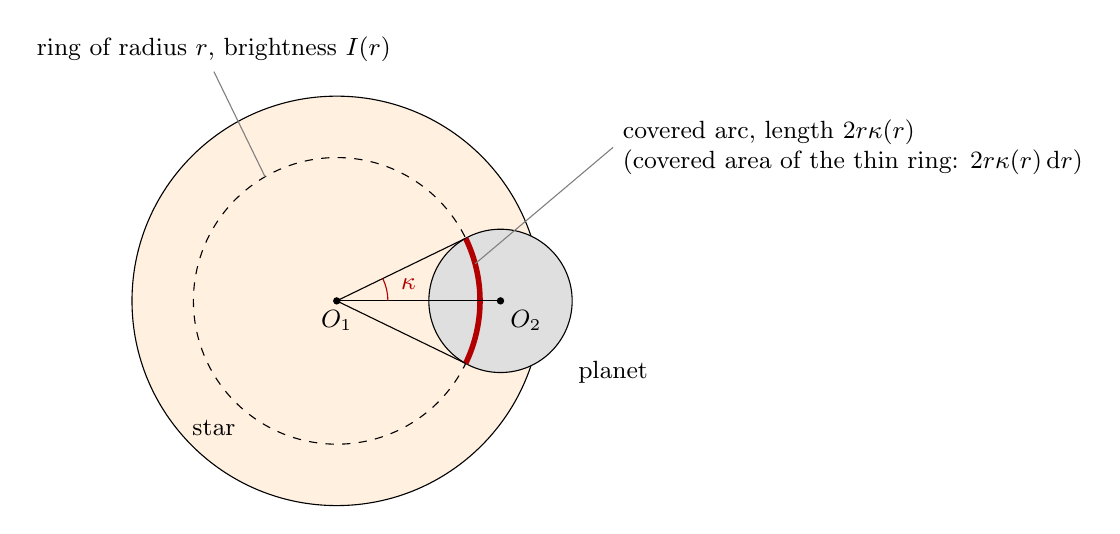
\begin{tikzpicture}[scale=2.6, font=\small]
    \pgfmathsetmacro{\lz}{0.8}
    \pgfmathsetmacro{\lp}{0.35}
    \pgfmathsetmacro{\lr}{0.7}
    \pgfmathsetmacro{\lk}{acos((\lr*\lr+\lz*\lz-\lp*\lp)/(2*\lr*\lz))}
    % star, ring, planet
    \fill[orange!12] (0,0) circle[radius=1];
    \draw (0,0) circle[radius=1];
    \draw[dashed] (0,0) circle[radius=\lr];
    \fill[gray!25] (\lz,0) circle[radius=\lp];
    \draw (\lz,0) circle[radius=\lp];
    % covered arc of the ring
    \draw[red!70!black, line width=2pt]
      ({\lr*cos(\lk)},{-\lr*sin(\lk)})
      arc[start angle={-\lk}, end angle=\lk, radius=\lr];
    % construction lines and the half-angle kappa
    \draw (0,0) -- (\lz,0);
    \draw (0,0) -- ({\lr*cos(\lk)},{\lr*sin(\lk)});
    \draw (0,0) -- ({\lr*cos(\lk)},{-\lr*sin(\lk)});
    \draw[red!70!black] (0.25,0) arc[start angle=0, end angle=\lk, radius=0.25];
    \node[red!70!black] at ({0.36*cos(\lk/2)},{0.36*sin(\lk/2)}) {$\kappa$};
    % centres
    \fill (0,0) circle[radius=0.018];
    \fill (\lz,0) circle[radius=0.018];
    \node[below] at (0,0) {$O_1$};
    \node[below right] at (\lz,0) {$O_2$};
    % labels
    \draw[gray] ({\lr*cos(120)},{\lr*sin(120)}) -- (-0.6,1.12)
      node[above, black] {ring of radius $r$, brightness $I(r)$};
    \draw[gray] ({\lr*cos(15)},{\lr*sin(15)}) -- (1.35,0.75)
      node[right, black, align=left] {covered arc, length $2r\kappa(r)$\\
      (covered area of the thin ring: $2r\kappa(r)\,\mathrm{d}r$)};
    \node at (-0.6,-0.62) {star};
    \node at ({\lz+0.55},-0.35) {planet};
  \end{tikzpicture}
  \caption{A ring of radius $r$ on the stellar disc, of uniform brightness
  $I(r)$. The planet covers an arc of the ring subtending the half-angle
  $\kappa(r)$ at the stellar centre $O_1$.}
  \label{fig:ring}
\end{figure}

\paragraph{Brightness.}
Brightness, or specific intensity, is
\begin{equation}
  I_\nu = \frac{\mathrm{d}E}{\mathrm{d}t \cdot \mathrm{d}A\cos\theta
          \cdot \mathrm{d}\Omega \cdot \mathrm{d}\nu},
\end{equation}
where
\begin{itemize}
  \item $\mathrm{d}E$ is the energy;
  \item $\mathrm{d}t$ is the time interval;
  \item $\mathrm{d}A\cos\theta$ is the projected area perpendicular to the ray,
        where $\theta$ is the angle between the surface normal and the ray;
  \item $\mathrm{d}\Omega$ is the solid angle (the direction of the ray);
  \item $\mathrm{d}\nu$ is the frequency interval.
\end{itemize}

\paragraph{Assumption.}
For limb darkening, the brightness at the same radius $r$ from the centre is
equal. So we can use the concept of a ring to compute the overall brightness
when an eclipse occurs.

\paragraph{Derivation.}
We have
\begin{equation}
  F(p,z) = 1 - \frac{\text{blocked brightness}}{\text{total brightness}}.
\end{equation}
We will use an integral where the radius $r$ slides from $0$ to $1$, and we
calculate the brightness blocked by the overlap on the ring at radius $r$ from
the centre and of width $\mathrm{d}r$. Since the total brightness comes from
full rings, each of length $2\pi r$,
\begin{equation}
  \text{total brightness} = \int_0^1 I(r)\, 2\pi r \,\mathrm{d}r .
\end{equation}

Now, let $\kappa(r)$ be the function returning the half-angle of the ring
fraction that holds the overlap at radius $r$ (Figure~\ref{fig:ring}). Then
\begin{equation}
  \text{blocked brightness}
  = \int_0^1 I(r)\, 2\pi r \cdot \frac{2\kappa(r)}{2\pi} \,\mathrm{d}r
  = \int_0^1 I(r)\, 2 r \kappa(r) \,\mathrm{d}r .
\end{equation}
Geometrically, from the cosine rule in the triangle formed by $O_1$, $O_2$
and an endpoint of the covered arc,
\begin{equation}
  \kappa(r) =
  \begin{cases}
    \pi, & r \le p - z
      \quad\text{(ring entirely inside the planet)}, \\[4pt]
    \cos^{-1}\!\left(\dfrac{r^2 + z^2 - p^2}{2 r z}\right),
      & |z - p| < r < z + p
      \quad\text{(ring crosses the planet's edge)}, \\[10pt]
    0, & \text{otherwise}
      \quad\text{(ring misses the planet)}.
  \end{cases}
\end{equation}

Hence we get our final relative flux formula:
\begin{equation}
  F(p,z) = 1 - \frac{\displaystyle\int_0^1 I(r)\, 2 r \kappa(r) \,\mathrm{d}r}
                    {\displaystyle\int_0^1 I(r)\, 2\pi r \,\mathrm{d}r}.
\end{equation}

% ---------------------------------------------------------------------------
\subsection{Orbital separation}
\label{sec:app-orbit}

Suppose $\omega = 2\pi/T$ is the orbital angular frequency ($T$ is the period),
$a$ is the orbital radius (circular orbit), and $t$ is the time measured from
mid-transit. What is $z(t)$? We need it to plot the light curve, the relative
flux $F(p,z)$ against time.

\begin{figure}[H]
  \centering
  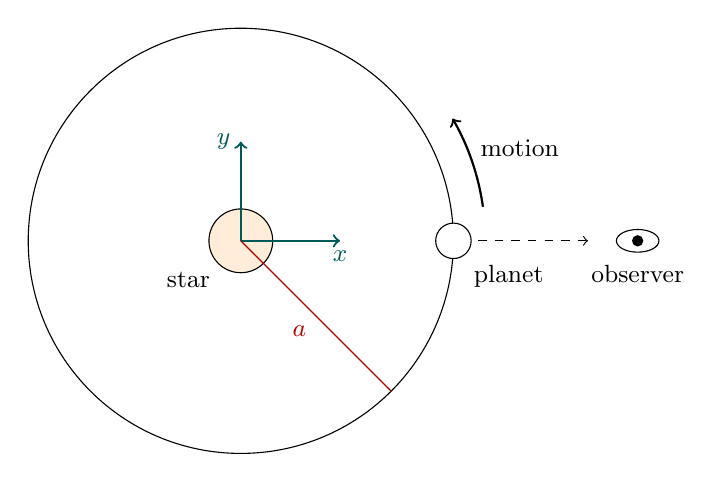
\begin{tikzpicture}[scale=0.9, font=\small]
    % orbit, star, planet
    \draw (0,0) circle[radius=3];
    \filldraw[fill=orange!15] (0,0) circle[radius=0.45];
    \filldraw[fill=white] (3,0) circle[radius=0.25];
    \node[below left] at (-0.3,-0.3) {star};
    \node[below right] at (3.15,-0.2) {planet};
    % direction of motion
    \draw[->, thick] (8:3.45) arc[start angle=8, end angle=30, radius=3.45];
    \node[right] at (22:3.5) {motion};
    % axes
    \draw[->, teal!70!black, thick] (0,0) -- (1.4,0) node[below] {$x$};
    \draw[->, teal!70!black, thick] (0,0) -- (0,1.4) node[left] {$y$};
    % orbital radius
    \draw[red!70!black] (0,0) -- ({3*cos(-45)},{3*sin(-45)})
      node[midway, below left] {$a$};
    % line of sight and observer
    \draw[->, dashed] (3.35,0) -- (4.9,0);
    \draw (5.6,0) ellipse[x radius=0.3, y radius=0.16];
    \fill (5.6,0) circle[radius=0.08];
    \node[below] at (5.6,-0.2) {observer};
  \end{tikzpicture}
  \caption{Top view of the orbit at mid-transit ($t = 0$). The observer lies
  on the $x$-axis, and the planet moves up (towards $+y$).}
  \label{fig:orbit-top}
\end{figure}

\begin{figure}[H]
  \centering
  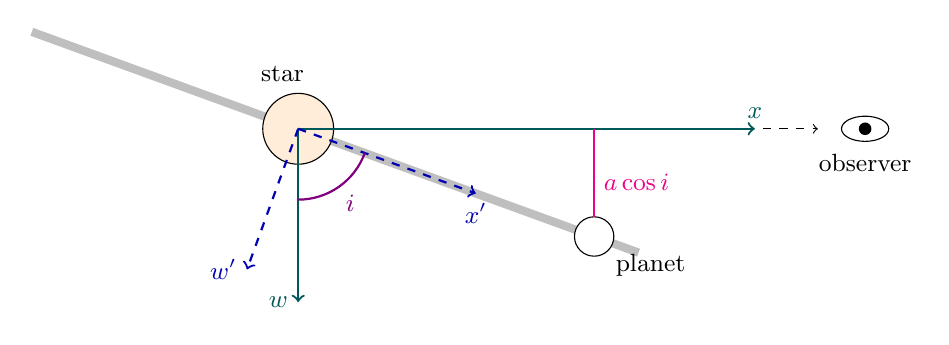
\begin{tikzpicture}[scale=1, font=\small]
    \pgfmathsetmacro{\inc}{70}
    \pgfmathsetmacro{\tilt}{90-\inc}
    % orbital plane seen edge-on
    \draw[gray, line width=3pt, opacity=0.5]
      ({-3.6*cos(\tilt)},{3.6*sin(\tilt)}) -- ({4.6*cos(\tilt)},{-4.6*sin(\tilt)});
    % star and planet
    \filldraw[fill=orange!15] (0,0) circle[radius=0.45];
    \filldraw[fill=white] ({4*cos(\tilt)},{-4*sin(\tilt)}) circle[radius=0.25];
    \node at (-0.2,0.7) {star};
    \node[below right] at ({4*cos(\tilt)+0.15},{-4*sin(\tilt)-0.1}) {planet};
    % sky-frame axes x (to observer) and w
    \draw[->, teal!70!black, thick] (0,0) -- (5.8,0) node[above] {$x$};
    \draw[->, teal!70!black, thick] (0,0) -- (0,-2.2) node[left] {$w$};
    % orbit-frame axes x' (in the orbital plane) and w' (orbit normal)
    \draw[->, blue!70!black, thick, dashed] (0,0) --
      ({2.4*cos(\tilt)},{-2.4*sin(\tilt)}) node[below] {$x'$};
    \draw[->, blue!70!black, thick, dashed] (0,0) --
      ({1.9*cos(-90-\tilt)},{1.9*sin(-90-\tilt)}) node[left] {$w'$};
    % inclination: angle between w and x'
    \draw[violet, thick] (0,-0.9) arc[start angle=-90, end angle={-\tilt}, radius=0.9];
    \node[violet] at ({1.15*cos(-45-\tilt/2)},{1.15*sin(-45-\tilt/2)}) {$i$};
    % w-coordinate of the planet at mid-transit
    \draw[magenta, thick] ({4*cos(\tilt)},{-4*sin(\tilt)+0.25}) -- ({4*cos(\tilt)},0);
    \node[magenta, right] at ({4*cos(\tilt)},{-2*sin(\tilt)}) {$a\cos i$};
    % observer
    \draw[->, dashed] (5.9,0) -- (6.6,0);
    \draw (7.2,0) ellipse[x radius=0.3, y radius=0.16];
    \fill (7.2,0) circle[radius=0.08];
    \node[below] at (7.2,-0.2) {observer};
  \end{tikzpicture}
  \caption{Edge-on view of the tilted orbit at mid-transit (drawn with
  $i = 70^\circ$). The orbit lies in the $x'$--$y$ plane, rotated about the
  $y$-axis (pointing out of the page); $i$ is the angle between the orbit
  normal $w'$ and the line of sight $x$, equivalently between $x'$ and $w$.}
  \label{fig:orbit-edge}
\end{figure}

I will operate with the real distance $d = z r_*$ for the derivation, then
divide by $r_*$ to get $z$.

\paragraph{Edge-on orbit.}
First, let us consider the simplest case, $i = 90^\circ$. Assume the planet in
Figure~\ref{fig:orbit-top} moves up, so if we plot its coordinates in the
$x$--$y$ plane, we get
\begin{align}
  x(t) &= a\cos\!\left(\tfrac{2\pi}{T} t\right) = a\cos(\omega t), \\
  y(t) &= a\sin\!\left(\tfrac{2\pi}{T} t\right) = a\sin(\omega t),
\end{align}
and, since the observer looks along the $x$-axis,
\begin{equation}
  d = |y(t)| = a\,|\sin(\omega t)| .
\end{equation}

\paragraph{Inclined orbit.}
Now we add the tilt (a rotation about the $y$-axis), which introduces the
third coordinate, $w$ (Figure~\ref{fig:orbit-edge}). In the
$(x', y, w')$ system, the coordinates are
$\bigl(a\cos(\omega t),\ a\sin(\omega t),\ 0\bigr)$. We need to convert them to
$(x, y, w)$. Since the observer sits on the $x$-axis, that coordinate is
irrelevant, so the answer will be $d = \sqrt{y^2 + w^2}$. The conversion gives
\begin{align}
  x' \to x &: \quad a\cos(\omega t) \;\to\; a\cos(\omega t)\sin i, \\
  w' \to w &: \quad 0 \;\to\; a\cos(\omega t)\cos i .
\end{align}
Therefore
\begin{equation}
  d(t) = \sqrt{a^2 \sin^2(\omega t) + a^2 \cos^2(\omega t)\cos^2 i}
\end{equation}
and
\begin{equation}
  z(t) = \frac{a}{r_*}\sqrt{\sin^2(\omega t) + \bigl(\cos(\omega t)\cos i\bigr)^2}.
\end{equation}

\paragraph{Note.}
This function gives exact values (including those for a transit) twice per
period. As we do not want to record a dip in flux when the planet is
\emph{behind} the star, we apply the constraint $\cos(\omega t) > 0$.

\subsection{Transit duration}
\label{sec:app-duration}

\subsection{The box-least-squares statistic}
\label{sec:app-bls}

\subsection{Period-grid spacing}
\label{sec:app-grid}

\subsection{Transit signal-to-noise}
\label{sec:app-snr}

\end{document}
